\subsection{Complex projective space $\CP{n}$}\label{sec-complex-projective-space}
The complex projective space, $\CP{n}$ is defined similarly to $\RP{n}$ as the space of complex lines in $\mathbb{C}^{n+1}$. Explicitly it is the quotient $\mathbb{C}^{n+1}\setminus \{0\}  \sim$ where $z\sim \lambda w$ for $\forall\lambda \in \mathbb{C}$. 

It is trivial to see that $\CP{0}\homeo\bullet$, as any $z\sim 1$ via multiplication by $\frac{1}{z}$. 

$\CP{1}$ is the quotient $\mathbb{C}^2/\sim,$
$$\begin{bmatrix} z\\ w \end{bmatrix}\sim \lambda \begin{bmatrix} z\\ w \end{bmatrix}.$$
If $w\neq 0,$ $$\begin{bmatrix} z\\ w\end{bmatrix}\sim \frac{1}{w}\begin{bmatrix} z\\ w\end{bmatrix}=\begin{bmatrix} z/w\\ 1\end{bmatrix}$$ We can relabel $u=z/w$, and note that any complex number can be written in this way. So $\{\begin{bmatrix} u\\ 1\end{bmatrix}\}\homeo \mathbb{C}\homeo \mathbb{R}^2$. The boundary (and complement) of this subset of $\RP{1}$ is the set $\{\begin{bmatrix} z\\ 0\end{bmatrix}\}/\sim\homeo \CP{0}\homeo\bullet$. Therefore $\RP{1}$ is the one-point compactification of $\mathbb{R}^2$, which homeomorphic to $S^2$. We can therefore give it a CW-complex structure of $1$ $0$-cell and $1$ $2$-cell, and its homology groups are the same as that of the $2$-sphere.

The general case can be done by induction.

\begin{prop}
As a cell complex, $\CP{n}$ has a $2m$-cell for $0<m\leq n$. As a consequence,
$$H_k(\CP{n})=\begin{cases} 
      \mathbb{Z} & k \text{ even, } 0\leq k \leq 2n \\
      0 & \text{otherwise}
   \end{cases}
$$
\end{prop}
\begin{proof}
We have proved the case $n=0,1$. In general, $\CP{n}=\mathbb{C}^{n+1}/\sim$
$$(z_1,z_2,\dots,z_{n+1})\sim \lambda (z_1,z_2,\dots,z_{n+1}), \lambda \in \mathbb{C}$$ If $z_{n+1}\neq 0$, we can let $\lambda=1/z_{n+1}$ to find a set of unique representatives
$$\{(u_1,u_2,\dots,1)\}\homeo C^{n}\homeo int(D^{2n}),$$
after relabeling $u_k=z_k/z_{n+1}$ for $0\leq k \leq n$.
The boundary (and complement) of this set in $\CP{n}$ is $$\{(z_1,z_2,\dots,z_n,0)\}/\sim \homeo \CP{n}$$ We can therefore give $\CP{n}$ the CW-structure of $\CP{n-1}$, with an additional $2n$-cell glued onto $\CP{n-1}$ by the projection on its boundary $p:S^{n-1}\rightarrow \CP{n-1}$. The result follows by induction. 

As $\CP{n}$ has no two $m$-cells in adjacent dimensions, its $m-th$ homology group is the free abelian group generated by its $m$-cell (or lack thereof).
\end{proof}
\begin{remark}\label{hopf}
It is worth looking at the gluing map of the 4-cell of $\CP{2}$ onto $\CP{1}\homeo S^{2}$. Via the homeomorphism, this is a map $S^{3}\rightarrow S^{2}$ with the property that the pre-image of every point is a great circle of $S^3$. This is because $\begin{bmatrix}z\\1 \end{bmatrix}\in \CP{1}$, chosen as a representative with norm $1$, is mapped to by $$\{\lambda \begin{bmatrix}z\\w \end{bmatrix} : \lambda\in \mathbb{C},|\lambda|=1\}\subset S^3\subset \mathbb{C}^2 ,$$ which is a great circle of $S^{3}$. This is exactly what characterises the famous Hopf map $h:S^3\rightarrow S^2$. Using the homeomorphism $S^3\homeo int(D^3)^*$ with the one-point compactification of the $3$-disk, the Hopf map can be visualised as in Figure \ref{hopf-fig}. The colours show which circles in $S^3\homeo int(D^3)^*$ are mapped to which points in $S^2$.
\end{remark}
\begin{figure}[h!]
    \centering
    \captionsetup{width=.7\linewidth}
    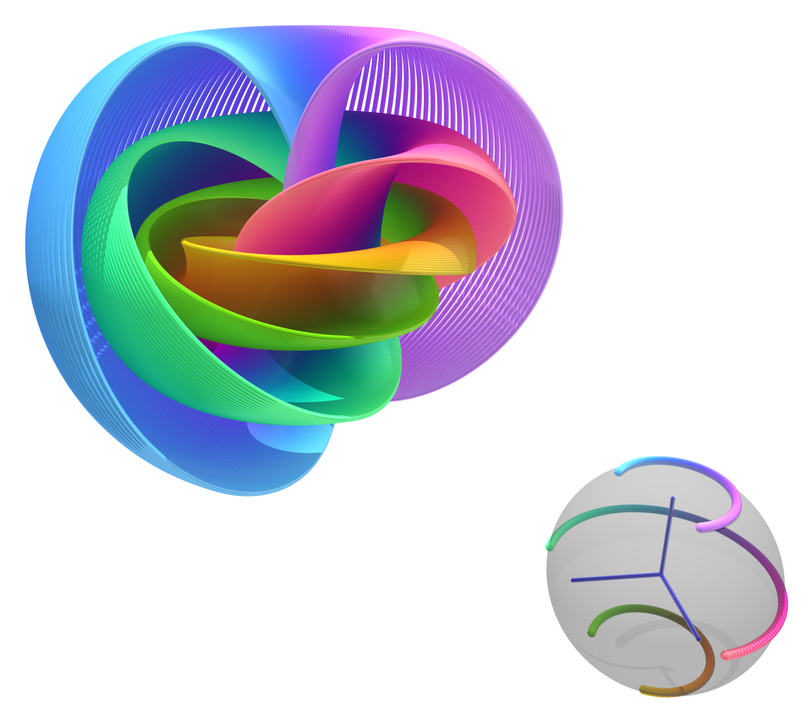
\includegraphics[width=0.5\textwidth]{hopf-fibration.png}
    \caption{The Hopf fibration. Image by Niles Johnson, CC BY-SA 3.0 \url{https://creativecommons.org/licenses/by-sa/3.0}, via Wikimedia Commons.}
    \label{hopf-fig}
\end{figure}
\subsection{Quaternionic projective space $\HP{n}$ and beyond}
The 2-dimensionality of $\mathbb{C}$ ensured that the n-cells of $\CP{n}$ were well spread in dimension, leading to an easy homology calculation. One can wonder if the higher-dimensional extensions of $\mathbb{R}$ are as easy to calculate, and indeed they are! The quaternions $\mathbb{H}$ is an extension of $\mathbb{R}$ homeomorphic to $\mathbb{R}^4$. It is \textit{not} a field, as it is not commutative. However, it retains all the other requirements of a field, importantly it has multiplicative inverses. Rings where every nonzero element has a multiplicative inverse are called \defn{division algebras}. The fact that $\mathbb{H}$ is a division algebra is what allows us to use the same argument as before on the Quaternionic projective space $\HP{n}$.

\begin{prop}
$\HP{n}$ has a cell structure with a $4k$-cell for $0\leq k\leq n$. As a consequence, $$H_k(\HP{n})=\begin{cases}\mathbb{Z} & k=0\text{ mod } 4 , 0\leq k\leq 4n \\ 0 & \text{otherwise}\end{cases}$$
\end{prop}

\begin{proof}
As in previous cases, $\HP{0}=\bullet$, as $z\sim 1$ for every $z\in \mathbb{H}$ by division by $z$. For general $\HP{n}$ we will proceed by induction. $\HP{n}=\mathbb{H}^{n+1}/\sim$
$$(z_1,\dots,z_{n+1})\sim h(z_1,\dots,z_{n+1}), \forall h\in \mathbb{H}.$$
If $z_{n+1}\neq 0$, we can divide by $z_{n+1}$ to find a set of unique representations
$$\{(u_1,\dots,u_n,1)\}\homeo \mathbb{H}^n\homeo int(D^{4n})$$
The boundary (and complement) of this set in $\HP{n}$ is the quotient 
$$\{(z_1,\dots,z_n,0)\}/\sim \homeo \HP{n-1}$$
We can therefore give $\HP{n}$ the CW-structure of $\HP{n-1}$, with an additional $4n$-cell mapped onto $\HP{n-1}$ via the projection on its boundary $p:S^{4n-1}\rightarrow \HP{n-1}$. By induction, $\HP{n}$ has the CW-structure stated in the proposition. Since $\HP{n}$ has no $m$-cells in adjacent dimensions, its $m$-th homology group is the free abelian group generated by its $m$-cell (or lack thereof).
\end{proof}

\begin{remark}
Notice that $\HP{1}$ has a 0-cell and a 4-cell, and is therefore homeomorphic to $S^{4}$. As in Remark \ref{hopf}, the gluing map of the 8-cell of $\HP{2}$ onto $\HP{1}\iso S^{4}$, therefore gives a "Hopf"-map $S^7\rightarrow S^4$ with the property that the preimage of a point is a "great" copy of $S^3$. If there was a way to keep extending $\mathbb{R}$ to a division algebra for every positive power of two we could repeat this process, yielding "Hopf"-maps from $S^{2^n-1}$ to $S^{2^{n-1}}$ for all $n>0$. However, this is false!!! The non-existence of such maps for $n>4$ proves there are no $2^n$-dimensional division algebras that extend $\mathbb{R}$ for $n>3$.
\end{remark}